\chapter{Reality and Models}
\label{ch:rm}

\section{Nature and Its Laws}
\label{sec:rm-nl}
\epigraph{Does the Moon exist only when somebody happens to be looking at it?}
{Albert Einstein}

Physics rests on a premise so basic that it is rarely stated out loud in
technical papers, and precisely because of that silence it is easy to lose
track of: \emph{Nature --- the physical universe --- is unique, and it
exists whether or not anyone is registering it.} The Moon orbited the Earth
for roughly four and a half billion years before any eye evolved capable of
noticing it. Electrons carried their charge and spin, atoms fused inside
stars, and galaxies wheeled through space long before there was a physicist,
a telescope, or a Geiger counter anywhere in the universe to say so. None of
that history was suspended for lack of an audience.

This is worth separating explicitly into two different things that everyday
language --- and, unfortunately, a great deal of popular writing about
physics --- routinely blur together:
\begin{description}
    \item [Physical reality:] what the universe and its constituents
  are actually doing, independent of anyone's knowledge of it.
    \item [ Our knowledge of physical reality:] the models, equations,
   and inferences by which we try to find out what physical
  reality is doing.
\end{description}

The first ---\emph{Real World} is presumed fixed and objective. It is unique
and exists independently of us. The observer who appears in physical literature
is nothing more than figure of speech. `Moon exists even nobody looks at it'
and so does electron. Real word objects behave according to Laws of Nature.
Contrary to human laws the Laws of Nature could never be violated. When we read
something like 'this device violates laws of physics' it means usually
misunderstanding or clickbait (probably both). Discovering of these laws is the
goal of physics. 

To achieve this goal we build the second --- \emph{Ideal World} which is
provisional, partial, and  is revised constantly --- and populate it by
mathematical models. These models emerge as result of  observations
(experiments, measurements, experience), their elements appear as ideal images
of real objects. Using instruments, which may be as simple as measuring tape or
lever scaling or as complex as electronic microscope or collider, experimental
physics gets facts of Real world. Theoretical physics constructs and update
mathematical models on base of these facts. It should be mentioned that our
instruments are part of Real world  and hence described by models\footnote{so a
person trying to disprove say quantum mechanics would have serious problem
since every modern instrument is based actually on quantum mechanics.}

Very instructive example of interaction between Real World and Ideal world
comes from astronomy.
When I was a student (more than 50 years ago), Pluto was officially counted as
the ninth planet. The change happened in 2006, when astronomers adopted a more
precise definition of what counts as a planet.
 
The problem arose because astronomers began discovering many objects beyond
Neptune, in the Kuiper Belt, some of them surprisingly large. In particular,
Eris, discovered in 2005, is nearly as large as Pluto.
This raised a difficult question:
If Pluto is a planet, should Eris also be a planet? And what about the other
large Kuiper Belt objects that might subsequently be discovered?
So in 2006 the International Astronomical Union (IAU) adopted a definition
requiring a body to satisfy three conditions to be a planet in our Solar
System:
\begin{enumerate}
   \item It orbits the Sun.
   \item It is massive enough for its own gravity to make it approximately round.
   \item It has cleared the neighborhood around its orbit of other objects.
\end{enumerate}
Pluto satisfies (1) and (2), but not (3). It lives in the Kuiper Belt among
many other objects of comparable orbital character.
Consequently, Pluto was reclassified as a dwarf planet, leaving eight planets:
Mercury – Venus – Earth – Mars – Jupiter – Saturn – Uranus – Neptune.

In fact, there is a rather amusing historical twist. Pluto was discovered in
1930, and its status as a planet was already somewhat unusual because it is
much smaller than the other planets. For decades this was not a serious problem
because no comparable objects were known.
Once the Kuiper Belt began to reveal itself, Pluto turned out to be the first
known member of a much larger population.

Nothing changed in Real World! Nothing physically happened to Pluto in 2006!
It did not become smaller, change its orbit, or somehow "lose" planetary
properties. The change was taxonomic: astronomers changed the definition of the
word "planet". New facts from Real World make us change our Ideal World!


\section{Models}
\label{sec:rm-mo}

When constructing a model, the following idealization is
made (see e.g. \cite{Arnold1998}): 
\begin{itemize}
    \item Events which are  highly probable in Real world become certain in ideal one.
    \item Plausible deductions become proofs.
    \item Some (irrelevant) details disappear.
    \item Approximate results become exact.
\end{itemize}               

This is how abstract notions such as perfectly rigid bodies, incompressible
fluids, material points, and so on emerge. Even the statement that results of
measurement are real numbers is actually idealization: no instrument is able to
produce output with infinite number of digits, hence experimental results are
always rational numbers.

When reasonable model is constructed, it is investigated and conclusions are
mapped back to Real world as predictions which should be tested by  experiment.
If we get  accurate description of reality the model remains {\em reasonable}
and can be foundation for other models, in particular those describing our
instruments, if not it  should be replaced or improved in some way or another.
If the model fails to produce results to be experimentally checked, it simply
makes no sense.

Let's assume that we have reasonable (mathematical) model. How can we obtain
correct conclusions from it. Purely formal reasoning risks gross errors.
Particularly dangerous is the temptation to demand precise  definitions for
every concept and object in a theory: such definitions often rest on seemingly
innocent assumptions whose physical meaning is unclear. As a result, one may
arrive at impeccably logical conclusions that nonetheless bear no relation to
the physical problem at hand.

Mathematical problems which required for physical predictions, except in the
simplest cases, are so complex that only approximate solutions are possible.
Often we cannot even verify the validity of the approximations we use, since
this would require exact solutions we cannot obtain. Actually we should use
some form of perturbation theory ---expansion in series over small
parameter(s). In most cases the convergence of the series is not proved (and
sometimes divergence is proved). Another way is numerical approach which of
course has its own pitfalls.

Here mathematician and physicist take different paths “The mathematician
proves, while the physicist convinces.” \cite{Medvedev2007}. Mathematician
rigorously and carefully investigates the model as it is formulated. Physicist
may change or abandon the model if it yields incorrect results (contradicting
to known experimental facts). Nature is too complex to be described by one
model. Physicist often uses more than one model simultaneously and change them
on the fly without warning or use some conditions which were not stated
explicitly. These tricks irritate mathematicians and confuse engineers. However
they are natural parts of physicist's way of thinking. 

\section{Coherence of Models}
\label{sec:rm-chm}

Contrary to what is said in many (good) books the relations among models are
not necessary hierarchical. Generally model may be a particular case of another
one only in restricted domain. For example only system of material points
interacting via electromagnetic or (and) gravitational field constitutes the
common subject of classical, relativistic and quantum mechanics and only for
such systems classical mechanics may be regarded as special case. Systems with
constraints generally can not be described in quantum or relativistic theory.

Physics advances largely by replacing complicated systems with
idealized limits: the point particle, the rigid body, the
continuum, the thermodynamic limit, the classical ($\hbar\to0$) 
and non-relativistic ($ c \to \infty $)
limits. These idealizations are so routine that it is easy to
forget they are genuine limiting procedures, valid only under
conditions that are rarely stated. When a system depends on a
single small (or large) parameter, sending that parameter to its
limiting value is usually harmless. Most interesting problems,
however, carry \emph{two or more} such parameters, and it is a
basic fact of analysis that iterated limits need not commute:
\[\lim_{\varepsilon\to0}\lim_{\delta\to0} f\]
can differ from
\[\lim_{\delta\to0}\lim_{\varepsilon\to0} f,\]
or the joint limit
may fail to exist at all. 

In modern physics, Berry is widely credited with cementing "singular limits" as
a major conceptual idea \footnote{I am aware of Arnold's Principle:
"Discoveries are rarely attributed to the correct person (including this
principle itself)"}. Berry extensively popularized the term to explain how
macro-scale "borderland physics" emerges from micro-scale laws (e.g., how wave
optics transitions to ray optics, or how quantum mechanics transitions to
classical chaos). But that word, by itself, is a label, not an explanation. Let
us consider some examples.

\paragraph{Calculus}
The phenomenon  already appears in
single-variable calculus applied to two variables. Consider
\begin{equation}
f(x,y) = \frac{x^2}{x^2+y^2}, \qquad (x,y)\neq(0,0).
\end{equation}
For any fixed $y\neq0$,
\begin{equation}
\lim_{x\to0}f(x,y)=0\longrightarrow\lim_{y\to0}\Big(\lim_{x\to0}f(x,y)\Big)=0,
\end{equation}
while for any fixed $x\neq0$,
\begin{equation}
\lim_{y\to0}f(x,y)=1\longrightarrow\lim_{x\to0}\Big(\lim_{y\to0}f(x,y)\Big)=1.
\end{equation}
The two iterated limits disagree, and in fact the joint limit
\[\lim_{(x,y)\to(0,0)}f(x,y)\]
does not exist at all: approaching
the origin along the ray $y=\lambda x$ gives 
\[f =1/(1+\lambda^2),\]
a different value for every slope $\lambda$.
There is no way to ``just set $x=y=0$''; the answer one gets
depends entirely on the \emph{path} by which the two small
parameters are sent to zero together, in other words the 
function is not analytical near $x=y=0$ point.

This is not a pathology invented for textbooks. It is the
generic behavior of a two-parameter limit unless one can show,
in addition to the two iterated limits agreeing, that the
convergence is \emph{uniform} -- that $f(x,y)$ is close to its
limiting value for \emph{all} small $(x,y)$ simultaneously, not
just along special directions. Physical idealizations are
exactly this kind of two-parameter limit whenever a problem
carries two small (or large) quantities -- a size and a
coupling, a compliance and a stiffness, an inverse system size
and a symmetry-breaking field -- that are both being sent to an
extreme value in the course of ``simplifying'' the problem.

\paragraph{Differential equations}
The same structure reappears, in disguise, in the classical
theory of \emph{singular perturbations}. Consider a
boundary-value problem such as
\begin{equation}
\varepsilon\, y''(x) + y'(x) = g(x), \qquad y(0)=y_0,\ \ y(1)=y_1,
\end{equation}
with $\varepsilon>0$ small. At $\varepsilon=0$ the equation
degenerates from second order to first order, and a first-order
equation cannot in general satisfy \emph{two} boundary
conditions. The naive limit ``set $\varepsilon=0$'' therefore
does not smoothly approach the true small-$\varepsilon$
solution: instead, the true solution develops a thin
\emph{boundary layer}, near one endpoint, across which $y$
changes rapidly to absorb the boundary condition that the
reduced ($\varepsilon=0$) equation cannot satisfy. Away from the
layer the reduced equation is an excellent approximation; inside
it, it is not. The parameter $\varepsilon$ multiplies the
\emph{highest derivative} in the equation, and it is precisely
this feature -- a small parameter multiplying the term that
carries the extra structure needed to fix an otherwise
under-determined problem -- that signals a dangerous limit. 

\paragraph{Geometry}
Take a right triangle with legs (catheti) of length $a$ and $b$, and hypotenuse
$c$ (see  Figure~\ref{stairs}). 
By Pythagoras,
$c=\sqrt{a^2+b^2}$. 

Instead of the straight hypotenuse, approximate it by a staircase: replace the
diagonal with a path that alternates horizontal and vertical steps, starting
at $(a,0)$ and ending at $(0,b)$. With $k$ steps, each horizontal segment has
length $a/k$ and each vertical segment has length $b/k$. Figure~\ref{stairs}
shows this staircase for $k = 1,2,4,8,16$, all overlaid on the same triangle,
together with the true hypotenuse in bold.

\begin{figure}[h]
\centering
\begin{tikzpicture}[scale=0.9]
\definecolor{tealA}{HTML}{9FE1CB}
\definecolor{tealB}{HTML}{5DCAA5}
\definecolor{tealC}{HTML}{1D9E75}
\definecolor{tealD}{HTML}{0F6E56}
\definecolor{tealE}{HTML}{085041}
\definecolor{coral}{HTML}{D85A30}

\newcommand{\staircase}[2]{%
  \pgfmathtruncatemacro{\kmax}{#1-1}
  \foreach \i in {0,...,\kmax} {
    \pgfmathsetmacro{\xa}{6*(1-\i/#1)}
    \pgfmathsetmacro{\ya}{6*\i/#1}
    \pgfmathsetmacro{\xb}{6*(1-(\i+1)/#1)}
    \pgfmathsetmacro{\yb}{6*(\i+1)/#1}
    \draw[#2, line width=0.9pt] (\xa,\ya) -- (\xb,\ya) -- (\xb,\yb);
  }
}
  % triangle
  \draw[gray, line width=0.8pt] (0,0) -- (6,0);
  \draw[gray, line width=0.8pt] (0,0) -- (0,6);
  \draw[gray, line width=0.6pt] (0.25,0) -- (0.25,0.25) -- (0,0.25);
  \node[below] at (3,0) {$a$};
  \node[left] at (0,3) {$b$};

  % staircases, coarsest to finest
  \staircase{1}{tealA}
  \staircase{2}{tealB}
  \staircase{4}{tealC}
  \staircase{8}{tealD}
  \staircase{16}{tealE}

  % true hypotenuse
  \draw[coral, line width=1.6pt] (6,0) -- (0,6);
  \node[coral, above right] at (3.3,3.3) {$c$};

  % legend
  \begin{scope}[shift={(0,-1.4)}]
    \draw[tealA, line width=0.9pt] (0,0) -- (0.5,0); \node[right, font=\footnotesize] at (0.55,0) {$k=1$};
    \draw[tealB, line width=0.9pt] (1.6,0) -- (2.1,0); \node[right, font=\footnotesize] at (2.15,0) {$k=2$};
    \draw[tealC, line width=0.9pt] (3.2,0) -- (3.7,0); \node[right, font=\footnotesize] at (3.75,0) {$k=4$};
    \draw[tealD, line width=0.9pt] (4.8,0) -- (5.3,0); \node[right, font=\footnotesize] at (5.35,0) {$k=8$};
    \draw[tealE, line width=0.9pt] (6.4,0) -- (6.9,0); \node[right, font=\footnotesize] at (6.95,0) {$k=16$};
  \end{scope}
  \begin{scope}[shift={(0,-1.9)}]
    \draw[coral, line width=1.6pt] (0,0) -- (0.5,0); \node[right, font=\footnotesize] at (0.55,0) {hypotenuse $c$};
  \end{scope}
\end{tikzpicture}
\caption{Staircases with $k=1,2,4,8,16$ steps between $(a,0)$ and $(0,b)$,
overlaid with the true hypotenuse (coral). As $k$ grows the staircase hugs
the diagonal ever more closely.}
\label{stairs}
\end{figure}

For every $k$, the horizontal segments of the staircase sum to exactly $a$
(they partition the base), and the vertical segments sum to exactly $b$.
So the total length of the $k$-step staircase is
$$L_k = a + b,$$
independent of $k$. As $k\to\infty$, the staircase converges pointwise to the
hypotenuse -- every point on it gets arbitrarily close to the diagonal line,
and the maximum distance between the staircase and the line is at most
$\max(a,b)/k \to 0$. Since the staircases ``become'' the hypotenuse in the
limit, and each one has length $a+b$, it seems to follow that
$$c = a+b.$$

The flaw is the assumption that if a sequence of curves converges to a limit
curve (as point sets, or uniformly), then their lengths converge to the
length of the limit. That assumption is false, and this staircase is the
standard counterexample.

One can think that paradox described above can
not occur for smooth curves, however even two smooth curve may coincide as sets of 
points, but have different lengths. Let $ y_n= \sin(n x)/n $ on the  
interval $ 0\le x \le 2 \pi $. Calculation of length of sinusoidal curve 
is a simple exercise in elliptic integrals:
\begin{equation}
   \label {sin-length}
   \begin{split}
       l_n&=\int_0^{2 \pi}\sqrt{1+\cos^2(nx)}dx\\
       &=\int_0^{2 n \pi}\sqrt{1+\cos^2(z)}dz/n\\
       &=\int_0^{2 \pi}\sqrt{1+\cos^2(z)}dz\quad \text{does not depend on n}  \\
       &=4 \sqrt{2} \int_0^{\pi/2}\sqrt{1-\frac{1}{2} \sin^2(z)}dz\\
       &=4 \sqrt{2} E(\frac{1}{\sqrt{2}}) \approx 1.351
   \end{split}
\end{equation}  
and ratio of its length to that of segment is $ \approx 1.22 $ independent of $
n $. On the other hand maximal distance between the curve and straight segment
$ d_n=1/n $ vanishes for $ n\rightarrow \infty $.

\paragraph{Algebra}
The Wigner--In\"on\"u contraction is a systematic procedure that produces one Lie
algebra as a singular limit of another.  Originally introduced by Wigner and
In\"on\"u, the method explains how nonrelativistic or
flat--space symmetry groups arise algebraically from relativistic or curved
ones.  The contraction operates entirely at the level of Lie algebras and does
not in general correspond to an isomorphism; it is a degeneration that reduces
the structure constants and typically turns a semisimple algebra into a
non-semisimple one.

Let $\mathfrak{g}$ be a Lie algebra with basis $\{X_i\}$ and commutation
relations
\begin{equation}
   [X_i,X_j] = f_{ij}{}^{k} X_k ,
\end{equation}
with constant structure coefficients $f_{ij}{}^{k}$.  A
Wigner--In\"on\"u contraction of $\mathfrak{g}$ is defined as follows:
\begin{enumerate}
\item Introduce a one--parameter family of invertible linear transformations
      $X_i \mapsto X_i(\varepsilon)$ for $\varepsilon \neq 0$.
\item Express the commutators in the $\varepsilon$--dependent basis:
\begin{equation}
    [X_i(\varepsilon),X_j(\varepsilon)]
        = f_{ij}{}^{k}(\varepsilon) \, X_k(\varepsilon).
\end{equation}
\item Take the limit $\varepsilon \to 0$, assuming it exists:
\begin{equation}
    \lim_{\varepsilon\to 0} f_{ij}{}^{k}(\varepsilon)
        = f^{(0)}_{ij}{}^{k}.
\end{equation}
\end{enumerate}
The algebra determined by $f^{(0)}_{ij}{}^{k}$ is called the
\emph{contracted Lie algebra} and is denoted $\mathfrak{g}_0$.

In the original formulation, $\mathfrak{g}$ is assumed to decompose as a vector
space into a direct sum
\begin{equation}
    \mathfrak{g} = \mathfrak{h} \oplus \mathfrak{p},
\end{equation}
where $\mathfrak{h}$ is a subalgebra.  One then rescales only the generators in
$\mathfrak{p}$:
\begin{equation}
   X_h' = X_h, \qquad
   X_p' = \varepsilon\, X_p,
\end{equation}
with $X_h \in \mathfrak{h}$ and $X_p \in \mathfrak{p}$.
Taking $\varepsilon \to 0$ yields the contracted algebra.

\paragraph{ The beam on three pillars}
Non-trivial limits may occur even at very simple mechanical
 problem. Let's take for example
a (rigid) beam on three (rigid) pillars (see fig.\ref{beam3}).

\begin{figure}[htbp]
    \centering
    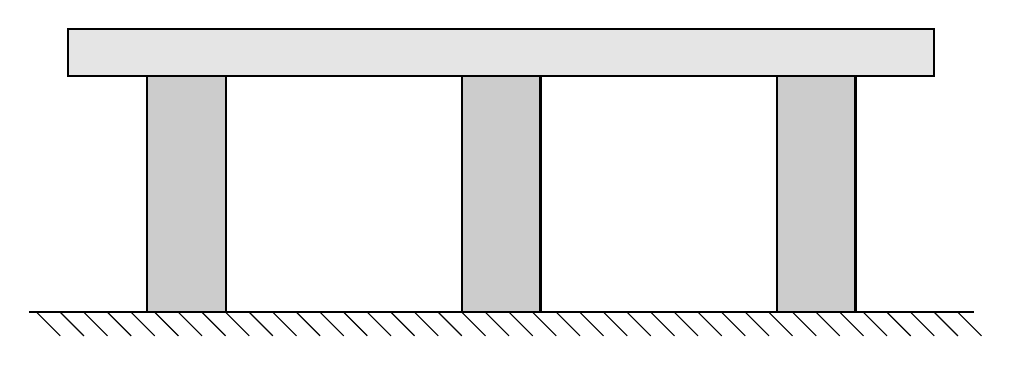
\begin{tikzpicture}[scale=1]
        % Beam
        \draw[fill=gray!20, thick] (0,3) rectangle (11,3.6);
        % Pillars
        \foreach \x in {1, 5, 9} {
            \draw[fill=gray!40, thick] (\x,0) rectangle (\x+1,3);
        }
        % Ground line
        \draw[thick] (-0.5,0) -- (11.5,0);
        % Ground hatching
        \foreach \x in {-0.4,-0.1,...,11.4} {
            \draw (\x,0) -- (\x+0.3,-0.3);
        }
    \end{tikzpicture}
    \caption{Beam resting on three pillars.}
    \label{beam3}
\end{figure}

Let the weight of the beam be $W$ and length $2 L$.
Balance of forces gives:
\begin{equation}
        F_0+F_1+F_2=W \label {bf}
\end{equation}
Balance of torques gives:
\begin{equation}
        F_1 L=F_2 L \label {bt}
\end{equation}
   So we have only two equations for three
unknown forces. From the symmetry we can get that $F_1=F_2$. 
(We know that this already from balance of torques.)
\begin{description}
    \item [First solution] All pillars and beam are absolutely rigid. Then
if we pull out the middle pillar nothing will change.
So $F_0=0$ and $F_1=F_2=W/2$.
    \item [Second solution] All pillars and beam are absolutely rigid. Then
we can cat beam at the center and will have two
beams laying on two pillars each.
So $F_0=W/2$ and $F_1=F_2=W/4$.
    \item [Third solution] Beam is absolutely rigid, pillars are very hard springs.
Since beam is horizontal, small change in length is 
equal to all pillars so $F_0=F_1=F_2=w/3$
    \item [Fourth solution] Pillars are rigid, beam is elastic. This case needs
some calculations, well known in elasticity theory
(see e.g \cite {LandauLifshitz-7}).
The results is $F_0=5 W/8$ and $F_1=F_2=3 W/16$.
It is clear that all these solutions (and more can be
produced) are limiting cases of standard elasticity 
problem when elasticity coefficients go to infinity.
\end{description}
So generally we can't simply neglect elastic deformations,
we should be more careful.

It is a piece of standard folklore, repeated in the first pages of countless
textbooks, that classical mechanics is ``what remains'' of relativity when
$c\to\infty$ (equivalently, when the characteristic speeds of the problem
satisfy $\beta = v/c \to 0$) and of quantum mechanics when $\hbar\to 0$. The
picture suggested by this way of speaking is a comforting one: there is a
single family of theories, continuously parametrized by $1/c$ and $\hbar$, with
special relativity and quantum mechanics sitting at generic points of the
family and classical mechanics sitting at the corner where both parameters
vanish. Classical mechanics, on this picture, is not really an autonomous
theory at all; it is a limit point, an image, a shadow cast by the deeper
theories onto the hyperplane $1/c=\hbar=0$.

 Two observations, already familiar to anyone who has tried to take the
folklore literally, show that something more interesting is going on.

First, the mathematical structures involved are not nested in the way the
picture requires. The phase space of a classical system and the Hilbert space
of its quantum counterpart are not the same kind of object related by a small
deformation; one is a symplectic manifold, the other a vector space with a
Hermitian form, and the passage between them (geometric quantization, or its
inverse) is a substantial piece of mathematics, not a Taylor expansion.
Likewise, the Galilei group is not a subgroup of the Poincar\'e group that one
recovers by ``turning off'' some generators. The relation between the
two is a \emph{contraction}, a specific and rather violent operation on Lie
algebras, not an inclusion.

Second, and more strikingly, classical mechanics contains objects that have no
counterpart at all on the other side of the limit, no matter how one takes it.
The rigid body is the standard example: an object whose configuration space is
finite-dimensional ($SE(3)$, or a quotient of it) precisely because every
internal distance is exactly conserved. Special relativity excludes such an
object outright, for any finite $c$, on causal grounds.

Friction and other dissipative forces are a second example: they break
time-reversal invariance and shrink phase-space volume, while the unitary
evolution of an isolated quantum system does neither, at any order in $\hbar$.
 These are not objects that quantum mechanics or
relativity describe badly, or only approximately; they are objects that
literally cannot be the image of anything on the quantum or relativistic side,
under any map deserving the name ``limit.''

The two observations reinforce each other. If the limit were regular --- if
solutions, symmetry groups, and observables all deformed continuously and were
connected by convergent, invertible correspondences --- then every classical
object would have to arise as the limit of \emph{something}, however
degenerate, on the quantum or relativistic side. The fact that some classical
objects have no such precursor is the symptom; the mismatch in mathematical
structure is the underlying disease. 

The right diagnosis is
that these are not (even singular) limits 
but something closer to an \emph{atlas} of local charts, each
valid in its own regime, glued together where their domains overlap, with no
single chart covering the whole territory.

Consider instead what it means for two maps to be maps ``of the same territory.''
Two maps can differ along at least four largely independent axes.

\paragraph{Theme: what a theory is about}

A weather map and a political map of France are not related by any limiting
procedure at all; neither is a coarsening or a refinement of the other, because
they depict different things. Mechanics, thermodynamics, and electromagnetism
stand in the same relation. Thermodynamics is not a low-resolution version of
electromagnetism, nor a special case of it; it is a different thematic layer
over the same territory, addressing questions (heat, entropy, equilibrium) that
a purely mechanical or electromagnetic map does not attempt to answer.
Demanding that thermodynamics arise as \emph{the} limit of electromagnetism
would be as confused as demanding that a weather map arise as the limit of a
political one.

\paragraph{Projection: how a theory represents its subject}

Within a single theme, different projections of the same territory preserve
different structure at the expense of other structure -- this is not a defect
of cartography but a theorem about it. A conformal (angle-preserving)
projection such as Mercator's cannot also be equal-area; an equal-area
projection such as Albers's cannot also be conformal. Gauss's \emph{Theorema
Egregium} makes the obstruction precise: a curved surface's intrinsic curvature
cannot be flattened into the plane without distorting either lengths, angles,
or areas -- there is no projection that gets everything right at once, only a
menu of projections each suited to a different purpose (Mercator for
navigation, Albers for area comparisons).

The different formalisms of a single physical theory are projections in exactly
this sense, not distinct theories and not limits of one another. The
Hamiltonian and Lagrangian formulations of classical mechanics carry the same
content but make different structure legible: the Hamiltonian picture displays
conserved quantities and symmetries transparently (as the book's chapter on the
geometric versus coordinate formulations of mechanics discusses at length)
while partially obscuring manifest covariance, which the Lagrangian picture,
built from a scalar action, preserves more readily. The Schr\"odinger,
Heisenberg, and path-integral pictures of quantum mechanics stand in the same
relation to one another. None of this is a reduction; it is re-projection, and
asking which picture is ``really'' the theory is as misguided as asking whether
Greenland is ``really'' as big as Africa.

\paragraph{Extent: domain of validity}

A street map of Paris does not contain Berlin, not because Berlin has been
idealized away but because it was never in scope. In the same way, Newtonian
gravitation's domain of validity (weak fields, low speeds) is a genuine subset
of general relativity's, and special relativity's domain (no gravity at all) is
neither contained in nor contains Newtonian gravity's domain -- the two extents
overlap only partially. This axis is what turns the whole picture from a loose
metaphor into something with real structure. 

\paragraph{Resolution: the one genuine limit, and why even it can fail}


Only along the resolution axis is ``limit'' close to the right word. A
1:1{,}000{,}000 map genuinely can, in principle, be produced by coarse-graining
a 1:1{,}000 map of the same theme, projection, and extent: this is a real
limiting operation on one and the same representation, and it is the
cartographic image of coarse-graining a microscopic statistical-mechanical
description into a macroscopic thermodynamic one, or of a renormalization-group
step integrating out short-distance degrees of freedom.

But even this limit routinely fails to be smooth. The length of a coastline,
measured at increasing resolution, does not converge to a finite number: it
grows without bound as the measuring scale shrinks, because coastlines are
statistically self-similar over a wide range of scales (the coastline paradox,
quantified by Richardson and Mandelbrot in terms of a fractal dimension greater
than one). Only certain coarse features -- the shape of a bay, the overall
outline of a continent -- stabilize under coarsening; the fine-grained quantity
``total length'' simply has no resolution-independent limit. The physical
analogue is exact: the thermodynamic limit is singular precisely at a phase
transition, where the system develops fluctuations at every length scale
simultaneously (critical phenomena), and the renormalization-group flow sits at
a fixed point at which ``resolution'' stops being a meaningful independent
parameter at all. The one axis along which cartography licenses talk of a limit
is also the one axis along which cartography itself warns that the limit can be
singular.

\paragraph{The discipline of atlas-making}

If this is right, the project of relating physical theories to one another is
better conceived as atlas-making than as limit-taking. An atlas does not aim at
a single chart covering everything -- indeed, for a sphere no such chart exists
without a coordinate singularity somewhere, a fact with the same flavor as the
no-go theorems. It aims instead at a well-chosen cover, with transition maps
that are explicit about where they are valid, honest about where they break
down, and unapologetic about the fact that some regions require an altogether
different theme, not merely a different resolution, to be represented at all.

This has the same shape as the real-world/ideal-world distinction developed in
Chapter~\ref{ch:rm}. A cartographic error occurs when a feature of the map -- a
projection's coordinate singularity at the pole, Greenland's inflated area
under Mercator -- is mistaken for a feature of the territory. The corresponding
physical error runs in both directions: treating the mathematical singularity
of a correspondence limit as if it were merely a calculational inconvenience to
be patched away, and, just as badly, dismissing a real emergent phenomenon that
appears only at the singularity of a limit -- a phase transition, a caustic,
the light cone itself -- as ``just'' an artifact of idealization. Both mistakes
come from forgetting that a map, however good, is not the territory, and that
the interesting places on any map are so often exactly where two of them stop
agreeing.

\section{The Return Path}
\label{sec:rm-rp}
\epigraph{Transfer of real object to ideal world
is not the same as transfer of ideal object to real world.}
{ V. Korneev (see \cite{StrugatskyStrugatsky2017})}.

Theoretical physics cannot be done without mathematics, but the relationship
between the two is instrumental, not devotional. Physics borrows notation,
structures, and inference rules from mathematics the way a carpenter borrows
tools from a hardware store: because they cut, join, and measure the material
actually in front of him. A tool earns its place in the workshop by what it
accomplishes there, not by how ingeniously it was machined. The question this
section asks is where the boundary of usefulness actually lies in the vast
modern mathematical toolkit --- which structures are cutting real material, and
which are being polished on the bench for their own sake and mistaken, by force
of habit, for physics.

Physicists like to invoke Wigner's observation about the unreasonable
effectiveness of mathematics as though it settled the matter for good:
mathematics simply works, so further scrutiny is unnecessary. Read carefully,
though, the effectiveness Wigner pointed to was narrow and specific --- a
comparatively small set of structures (calculus, linear algebra, differential
geometry, group representations) turned out to fit an equally specific set of
physical problems astonishingly well. That is a track record, compiled piece by
piece over three centuries, not a blank check issued to every mathematical
structure a theorist happens to find beautiful. Each new import from pure
mathematics has to earn its keep on its own; none inherits Newton's or
Einstein's credit automatically.

The previous section drew a line between the Real Word of causal processes and
experimentally accessible phenomena, and the Ideal Word of mathematical models
a physicist constructs to represent it. Causality and experimental support are
properties of the real world; logical construction and internal consistency are
properties of the ideal world; confusing the two registers is what generates
paradoxes.

That distinction supplies the criterion this section needs. Call the
\emph{return path} the interpretive dictionary --- however indirect --- that
connects some object or relation in the ideal world back to a causal or
measurable feature of the real world. A piece of mathematics belongs in
theoretical physics for exactly as long as such a dictionary exists and keeps
being used, not merely gestured at.

Newton's second law: 
\[m\ddot{x} = F(x,t),\] 
the heat equation: 
\[\partial_t u =\kappa\,\nabla^2 u,\] 
and the wave equation:
\[\partial_t^2 u = c^2\,\nabla^2 u,\]
are the paradigm of useful mathematics because they were not imported into
physics; they were extracted from it. Every symbol carries an operational
meaning fixed independently of the equation itself --- mass and force are read
off a scale and a spring, $u$ is a temperature read off a thermometer, boundary
conditions are the literal edges of the physical body in question. Solving the
equation issues a prediction that a second, independent measurement can confirm
or refute. The return path is not an afterthought; it is built into the
vocabulary before the first derivative is taken.

This does not make differential equations safe as a category. The modern theory
of PDEs, pursued as pure analysis, ranges deep into existence and uniqueness
results in exotic Sobolev and Besov spaces that no experiment will ever probe.
Even inside the paradigm case there is a gradient of physical relevance. What
keeps the tool tethered is not the label ``differential equation'' but the
discipline of keeping the interpretation live at every step --- checking, at
each manipulation, that the symbols still point at something a real-world
measurement could in principle confirm.

\section{Structures Without a Return Path}
\label{sec:rm-nrp}
\paragraph{Category Theory and Topos Theory }
Category theory studies objects only through their morphisms and the ways
morphisms compose; a functor $F: \mathcal{C} \to \mathcal{D}$ carries this
relational skeleton from one category to another while preserving composition,
so that a square of morphisms
\[
\begin{tikzcd}
A \arrow[r, ] \arrow[d, '] & B \arrow[d, ] \\
C \arrow[r, '] & D
\end{tikzcd}
\]
commutes. It is one of the great
structuralist achievements of twentieth-century mathematics: a language for
talking about \emph{structure of structures}, deliberately abstracted away from
any particular set of objects. Topos theory generalizes this further, replacing
the category of sets itself with a more general universe of ``variable sets''
equipped with its own internal logic.

Physics has borrowed both. Categorical quantum mechanics recasts quantum
processes as morphisms in a compact closed category, with entanglement and
measurement drawn as string diagrams. The topos approach to quantum theory
reformulates quantum logic using presheaves over a category of experimental
contexts, in an effort to remove the privileged classical observer from the
axioms. Both programs are technically serious and internally elegant.

What neither program has yet produced is a new number: no categorical or
topos-theoretic reformulation has predicted an observable that the
Hilbert-space formalism it re-describes did not already predict. The
translation runs ideal-world to ideal-world --- from one formal language to a
more abstract one --- without a new leg reaching back into the real world. By
the criterion of this section that makes the apparatus, at present, ornamental
with respect to physics, whatever its merits as foundations or as mathematics
in its own right. The verdict is about the current absence of a return path,
not about abstraction as such, and it is explicitly revisable if that path is
ever found.

\paragraph{Berezin's Supermathematics }
Grassmann numbers anticommute, $\{\theta_i,\theta_j\}=0$, and Berezin
integration is defined algebraically rather than as a limit of sums:
\[
\int d\theta\,\theta = 1, \qquad \int d\theta\, 1 = 0 .
\]
This machinery exists to give fermionic path integrals a well-defined meaning:
anticommuting $c$-numbers are exactly what is needed to reproduce the minus
sign attached to a closed fermion loop, and through it the Pauli exclusion
principle that keeps ordinary matter from collapsing. That minimal core is
squarely inside the boundary --- its consequences are checked every time a
collider experiment counts fermion loops correctly.

Superspace is a further, larger step. It promotes the anticommuting variables
to new coordinates $(x^\mu,\theta^\alpha,\bar\theta_{\dot\alpha})$ alongside
ordinary spacetime, so that a supersymmetry generator can shift a boson into a
fermion,
\[
\{Q_\alpha, \bar Q_{\dot\beta}\} = 2\,\sigma^\mu_{\alpha\dot\beta}\,P_\mu ,
\]
and superfields package whole supermultiplets into a single object defined over
this extended space. No clock or ruler has ever read a value of $\theta$; the
extra coordinates are motivated by the elegance of unifying bosons and fermions
and by the divergence cancellations supersymmetry provides, not by any
operationally required content. Direct searches at the LHC have found no
superpartners at the energies once expected to reveal them, and the naturalness
argument that motivated a low-mass spectrum has been pushed to ever higher,
less testable scales with each null result --- the return path, already thin,
has been thinning further for two decades. The Grassmann bookkeeping stays; the
spacetime extension it was generalized into remains, so far, a construction
that lives entirely in the ideal world.

\paragraph{String Theory's Mathematical Apparatus }
Compactifying the extra dimensions of string theory on a Calabi--Yau manifold,
tracking how its complex and K\"ahler moduli vary, and matching pairs of
manifolds under mirror symmetry is one of the genuine triumphs of
late-twentieth-century mathematics: physical reasoning about string worldsheets
led directly to theorems in enumerative algebraic geometry, including exact
counts of curves that had resisted purely mathematical attack. Branes,
correspondingly, are understood as objects in the derived category of coherent
sheaves. As an engine for producing new, provable mathematics, the apparatus is
an unqualified success.

As physics, the diagnosis is different. Compactification does not pick out a
single vacuum; it generates a landscape estimated at roughly $10^{500}$
consistent possibilities, each with its own low-energy constants. A structure
flexible enough to accommodate almost any observed set of constants after the
fact has stopped constraining the real world in advance, and the capacity to be
wrong in advance is exactly what a return path is for. This is the same
category error the previous section located in Hempel's paradox, transplanted
from a single model onto a landscape of them: mathematical existence and
internal consistency, however large and beautifully classified the resulting
catalogue, are being read as physical relevance, when nothing yet says which
entry in the catalogue --- if any --- is the real world's.

\section{Measurements}
\label{sec:rm-me}

\epigraph{``We do not know what space, time, and motion are --- 
but we know how to measure them.''}{R. Feynman}

Actually the sentence in epigraph  is not a single line Feynman wrote down; it
is the working motto of physics itself, and Feynman stated its three parts
separately, in three different lectures, about three different things. This
section tells that story and asks what it means for the rest of the subject you
are about to study.

Open almost any introductory physics course and you will be handed, within the
first few pages, definitions of space, time, and motion. You will be told that
time is ``what a clock measures,'' that length is ``what a ruler measures,''
and that velocity is ``the rate of change of position.'' If you find these
definitions strangely circular --- clocks measure time, but what \emph{is}
time? --- you are in good company. So did Richard Feynman, and so did every
serious physicist since Galileo.

In the opening lectures of \cite{flp1}, Feynman
confronts this circularity head-on, not once but three times, for three
different concepts.

On \textbf{energy}, in a lecture on its conservation, he is blunt: it is
important to realize that in physics today, he says, ``we have no knowledge of
what energy is'' --- we only have formulas that let us calculate a number,
before and after some process, and find that the number has not changed.

On \textbf{time}, wrestling with the fact that no dictionary definition of time
is any good (Webster's circles back on itself), he concludes that what matters
is ``not how we define time, but how we measure it'' --- and spends the rest of
the lecture on clocks, not metaphysics.

On \textbf{motion} and definition generally, after a philosophical detour about
whether a moving object is the ``same'' object from moment to moment, he throws
up his hands in a way every working scientist will recognize: ``We cannot
define anything precisely!'' What rescues physics from paralysis, he goes on,
is that we do not need a precise definition of a \emph{thing} in order to make
precise \emph{measurements} of it.

Actually to measure thing we need some
system of units. What is good about units is that there is plenty of choices.
SI system is the most popular. In this system, as described by NIST (National
Institute of Standards and Technology, US), seven base units are defined.
\begin{description}
    \item [time] 
        The second (s) is defined by taking the fixed numerical value of the
        unperturbed ground-state hyperfine transition frequency of the
        cesium-133 atom, to be 9,192,631,770 when expressed in the unit Hz,
        which is equal to \unit{ s^{-1}}.
    \item [length] 
        The meter (m) is defined by taking the fixed numerical value of the
        speed of light in vacuum c to be 299,792,458 when expressed in the unit
        \unit{m.s^{-1}}.
    \item [mass] 
    The kilogram (kg) is defined by taking the fixed numerical value of the
        Planck constant h to be $6.62607015 10^{-34}$ when expressed in the
        unit \unit{J.s}, which is equal to \unit{kg.m^2.s^{-1}}.
    \item [electric current] 
    The ampere (A) is defined by taking the fixed numerical value of the
        elementary charge e to be \num{1.602176634e-19} when expressed in the
        unit C, which is equal to \unit{A.s}.
    \item [temperature] 
    The kelvin (K) is defined by taking the fixed numerical value of the
        Boltzmann constant k to be \num{1.380 649e-23} when expressed in the
        unit \unit{J.K^{-1}}.
    \item [amount of substance] 
    Mole (mol) contains exactly \num{6.02214076e23} elementary entities. This
        number is the fixed numerical value of the Avogadro constant, NA, when
        expressed in the unit \unit{mol^{-1}}.
    \item [luminous intensity] 
    The candela (cd) is defined by taking the fixed numerical value of the
        luminous efficacy of monochromatic radiation of frequency num{540e12}
        Hz, Kcd, to be 683 when expressed in the unit \unit{lm.W^{-1}}, which
        is equal to \unit{cd.sr.W^{-1}}.
\end{description}
Last three units have no use in theoretical physics and are mentioned for 
completeness only.

If restricted to length,time and mass all systems of units  differ only by
scale and hence using of this or that system is a matter of taste. For
example,to demonstrate good education, one can use 'FFF system' --- Furlong as
unit of length (201 m), Firkin(of water) as unit of mass (41 kg), and Fortnight
as unit of time ($ 14\times 86400 s $). 

The situation is more complicated when when we consider electromagnetic
phenomena. SI introduces amper as independent unit which allows to use familiar
units for voltage, current and so on. However the price for that is too high,
dimensional permeability of vacuum emerges, components of electromagnetic field
are measured with different units etc. So I shall use Gaussian system, time is
measured in seconds, length in centimeters, and mass in grams. Unit of charge
is defined so that Coulomb low is written as \[ U= \frac{q_1 q_2}{r} \] so its
dimension is \unit{g^{1/2}.cm^{3/2}.s^{-1}}. 

Anyway, despite of efforts of proponents of SI, a number of external units is
popular in practice. In elementary particle physics energy is mostly measured
in electron-volts (\unit{eV}) which is equal to  \num{1.602176634e-19} J, while
in power engineering  in kilowatt-hours (\unit{kW}) equal to \num{3.6e6} J.

Sometimes simple change of units allows better understanding. For example, 
how high are energies in High Energy Physics? --- Simple calculation shows
 that kinetic energy of flying mosquito is approximately 4
\unit{TeV}. How mach energy contains macroscopic body in rest? ---
Total electric energy produced in US in 2022 is approximately
\num{1.6e19} J, which correspond to approximately 200 \unit{kg} according to $
E=m c^2 $ formula.

\section{Physics is not Data Science}
\label{sec:rm-pds}

\epigraph{Not being able to define a thing precisely is not the same failure 
as not understanding it.}{ R. Feynman}
 Physics survives without precise definitions because it replaces them with
 measurement procedures. This chapter argues that measurement procedures are
 the \emph{floor} of physics, not its ceiling --- and that the gap between the
 floor and the ceiling is exactly what separates a physicist from a
 curve-fitting algorithm.

The claim in the epigraph above rests on two sentences Feynman actually said,
in different lectures, about different things -- and they are routinely
collapsed into one. They should not be.

``We cannot define anything precisely'' was said about ordinary words like
\emph{motion} -- a confession that physics does not wait for philosophical
certainty about what a thing \emph{is} before it starts measuring it precisely.
That is an epistemic strategy: start with measurement, because measurement is
checkable and definition-by-essence is not.

``I think I can safely say that nobody understands quantum mechanics'' was said
in a completely different spirit.  Feynman had just finished pointing out that
although newspapers once claimed only twelve people understood relativity, that
was never really true --- once Einstein's paper was published, plenty of people
came to understand it, in the ordinary sense of being able to picture what it
says. Quantum mechanics, he then says, is different: nobody has ever been able
to reduce it to a picture built out of everyday experience, the way you can
eventually picture curved spacetime with enough effort. That is not a statement
that physicists cannot use quantum mechanics, predict with it, or reason about
it --- they do all three, correctly, every day, and Feynman himself spent the
rest of that same lecture doing exactly that. It is a much narrower claim: no
one has found a \emph{classical, intuitive mechanism} underneath it.
Understanding, in that specific and demanding sense, is missing. Understanding
in the working sense --- knowing the structure, deriving its consequences,
trusting it enough to build a transistor or a laser on top of it --- is not.

This section is about the difference between those two kinds of understanding,
and about a claim worth taking seriously: that pure operationalism, on its own,
cannot tell them apart. If all that mattered were successful measurement and
prediction, there would be no principled way to say that a physicist
understands gravity more deeply than a weather-prediction algorithm understands
rain. Physics needs, and has, a further standard.

Return to  account of measurement. An operational definition says: a quantity
is whatever a specified procedure outputs. This is enough to make a concept
scientific --- checkable, shareable, free of unfalsifiable metaphysics. It is
not enough, on its own, to distinguish two very different kinds of success.
\begin{enumerate}
\item A theory that predicts a measurement because it encodes something
    structural about how the world is put together: a small number of
        principles from which the measured value can be \emph{derived}.
\item A model that predicts a measurement because it has been fitted, with
    enough free parameters, to enough past instances of that same measurement,
        with no claim about structure at all.
\end{enumerate}

Operational equivalence in the old domain said nothing at all
about generative power in the new one. That gap is what
\emph{understanding} means in physics. It is not merely getting
today's number right. It is possessing a formulation with enough
internal structure that it tells you, in a principled way, what
to try next.

A purely operational, purely data-fitted model was built to reproduce association between
measurement and measurement, and nothing in its construction licenses a claim
about what would happen under conditions it has never seen. A physical theory
with real structure --- Newton's law derived from a principle, not merely
fitted to Tycho Brahe's tables ---  tells you what happens if you change the mass
of the Sun (in equations, of course),
\footnote{This makes sense for example if you are trying
to figure out the fate of solar system when Sun will lose enough mass due 
to radiation.}
a question no data set has ever answered, because the answer is
derivable rather than looked up.

This is the precise place where physics and data science part ways, and it is
worth stating the comparison without exaggerating it in either direction.

Train a sufficiently flexible statistical model on centuries of recorded
planetary positions and it will predict tomorrow's positions beautifully ---
quite possibly to a precision rivaling Newton's own equations, for exactly the
regime it was trained on. It has, in the fullest operational sense, learned to
measure and predict planetary motion. What it has not done is acquire a reason
to trust its own output the moment the situation changes: a new comet on a
hyperbolic orbit, a spacecraft under active thrust, a binary star system where
the gravitational field is far stronger than anything in the training data. A
model built on correlation has no internal signal that it has left its depth
--- it will output a confident number regardless. Newton's law, by contrast,
comes with a built-in structure, which allows to check where and why it should be
expected to fail: at speeds approaching $c$, or fields strong enough that
spacetime curvature can no longer be neglected. Knowing your own boundary of
validity is itself a form of understanding, and it is precisely what falls out
of having a mechanism rather than a fit.

None of this makes data-driven methods unscientific, and it would be a mistake
to read this section that way. Statistical inference is indispensable precisely
where no mechanistic theory yet exists, and some of the most interesting
current work in physics itself uses machine learning as a tool for discovery
--- to search for patterns in particle-collider data, or in gravitational-wave
signals, that a human physicist might not think to look for. Tellingly, though,
the most physically successful of these tools are increasingly built to encode
known structure directly --- conservation laws, symmetries, the least-action
principle itself --- rather than learning everything from scratch. That design
choice is itself an admission of this section's argument: bare correlation
extrapolates badly, physicists are to find the formulation that carries 
structure, not just the one that fits the numbers.

Section~\ref{sec:rm-me} started with a motto built from three of
Feynman's remarks: physics
does not need to know what space, time, or motion \emph{are}, only how to
measure them. That motto is correct as far as it goes, and it is where physics
has to start. This section has argued that it is not where physics is content
to stop.

A physicist who has only an operational definition and an accurate prediction
has done real, indispensable work. A
physicist who additionally has a structure --- a small set of principles from
which that prediction, and a thousand others never yet measured, can all be
derived --- has done something further, and it is that further thing which
earns the word \emph{understand}. The motto of this chapter is the necessary
second half of the first:

\emph{We measure a thing before we understand it. We understand it once our
account of it lets us predict what we have never measured at all.}


\section{The Physicist as Intuitive Bayesian}
\label{sec:rm-pib}

A physicist does not confront data from a position of ignorance. Before a
single measurement is taken, she has already restricted attention to a family
of models $\{M_\theta : \theta \in \Theta\}$ --- Newton's law with an unknown
spring constant, a resonance of unknown mass and width, a cosmological model
with unknown $\Omega_\Lambda$. This restriction is not neutral. It is an act of
assigning prior plausibility zero to the overwhelming majority of functions
that could in principle be fit to any given data set, and non-negligible
plausibility to a small, structured subset selected by symmetry,
renormalizability, dimensional analysis, or simply what has worked before. This
is the content of a Bayesian prior, whether or not it is ever written as
$\pi(\theta)$. The thesis of this section is that physics, as actually
practiced, is Bayesian inference over a self-imposed model space --- even when,
and especially when, the explicit statistical vocabulary used to report the
result is frequentist.

\paragraph{Model space as an implicit prior}

\begin{definition}
A \emph{model space} $\mathcal{M}$ is the set of hypotheses a physicist is
    willing to entertain prior to seeing the data at hand, together with a
    measure $\pi$ of relative plausibility over that set --- possibly only
    ordinal, and rarely written explicitly.
\end{definition}

Formally, inference within a chosen model proceeds by
\begin{equation}
P(\theta \mid D, M) \;=\; \frac{P(D \mid \theta, M)\,\pi(\theta \mid M)}
    {\displaystyle\int_{\Theta} P(D \mid \theta', M)\,\pi(\theta' \mid M)\, d\theta'}
    \,, \qquad \theta \in \Theta_M,
\end{equation}
but the physicist's real act of judgment happens one level up, in the choice of
$M$ itself from the space of all conceivable models $\mathcal{M}$. Requiring
Lorentz invariance, gauge invariance, renormalizability, or simply a low-order
polynomial in the fields are all instances of setting $\pi(M') = 0$ for models
$M'$ outside the chosen family --- an extremely informative prior, imposed
before any likelihood is ever evaluated, and rarely defended in the
probabilistic language it deserves.

\begin{remark}
Occam's razor, as actually practiced in theoretical physics --- preferring the
    model with fewer free parameters, absent a specific reason to prefer
    otherwise --- is not a separate methodological principle standing outside
    probability theory. It is a description of a prior that penalizes model
    complexity, and it has a standard formal counterpart in Bayesian model
    comparison: the automatic Occam penalty carried by the marginal likelihood
\begin{equation}
P(D \mid M) \;=\; \int_{\Theta} P(D \mid \theta, M)\,\pi(\theta \mid M)\, d\theta,
\end{equation}
which is suppressed for models whose parameter space wastes prior mass on
    regions the data rule out.
\end{remark}

\paragraph{Sequential updating across experiments}

The history of confidence in General Relativity is not well described as a
sequence of independent frequentist tests, each beginning from total ignorance
and returning a verdict discarded once the next experiment starts. Each
successive test --- Mercury's perihelion, light bending, gravitational
redshift, binary-pulsar timing, the direct detection of gravitational waves ---
is treated as tightening an already substantial body of belief, and a single
anomalous result is weighed \emph{against}, not substituted for, everything
already established. This is posterior-to-prior updating,
\begin{equation}
\pi_n(\theta) \;\propto\; P(D_n \mid \theta)\,\pi_{n-1}(\theta),
\end{equation}
carried out informally, paper by paper, over decades, whether or not any
individual paper ever computes a posterior.

\paragraph{Confidence intervals: frequentist construction, Bayesian use}

A frequentist $100(1-\alpha)\%$ confidence interval $I(D)$ is defined by the
coverage property
\begin{equation}
P_\theta\big(\theta \in I(D)\big) = 1-\alpha \qquad \text{for every fixed } \theta,
\end{equation}
a statement about the behavior of the \emph{procedure} across a hypothetical
ensemble of repetitions of the experiment at the same true $\theta$. By
construction it makes no probabilistic statement about whether the true value
lies in the one particular interval actually obtained from the one experiment
that was run.

\begin{remark}
This is almost never how such an interval is read once quoted. ``The top-quark
    mass is $172.5 \pm 0.7\ \mathrm{GeV}$'' is universally understood,
    including by the physicists reporting it, as licensing something close to
    ``there is roughly a 68\% chance the true mass lies in this range'' --- a
    statement about degree of belief in a fixed but unknown constant,
    conditioned on the one data set actually obtained. That is a Bayesian
    credible interval, not the frequentist object formally computed. The two
    coincide numerically under a flat prior in a wide class of problems, which
    is precisely why the conflation goes unnoticed.
\end{remark}

\paragraph{Systematic uncertainty as a nuisance-parameter prior}

A detector's calibration constant, an integrated luminosity, a background
normalization --- these are not resampled across hypothetical repetitions of
the universe; they are fixed, unknown quantities specific to the one apparatus
and the one run at hand. Assigning them an error distribution and
marginalizing,
\begin{equation}
P(\theta \mid D) \;=\; \int P(\theta \mid D, \lambda)\,\pi(\lambda)\, d\lambda,
\end{equation}
over a nuisance parameter $\lambda$ --- calibration, background rate,
theoretical cross-paragraph uncertainty --- is exactly Bayesian
nuisance-parameter marginalization. There is no frequentist repeated-sampling
story under which ``the calibration constant of this detector, on this day, has
a 90\% confidence interval'' is a meaningful statement: there is only one
calibration constant, and one day. Experimental physicists carry out this
marginalization routinely, correctly, and almost never under that name.

\paragraph{Case study: the $5\sigma$ threshold and the Higgs boson}

The 2012 discovery announcement was couched entirely in frequentist terms: a
local significance in excess of $5\sigma$, i.e.\ a $p$-value under the
background-only null hypothesis below roughly $3\times10^{-7}$. This is, by
construction, \emph{not} a posterior probability that the Higgs boson exists,
and not a statement about $P(\text{Higgs} \mid D)$ at all --- a point
statisticians raised at the time and which physicists mostly reasoned past
rather than through.

\begin{remark}
What made the announcement compelling was never the $p$-value in isolation. It
    was the $p$-value combined with decades of prior theoretical commitment ---
    electroweak precision fits, unitarity arguments against a Higgsless
    Standard Model, a mass window already narrowed by indirect constraints ---
    that gave the community a strong prior concentrated near the observed mass
    before ATLAS and CMS reported anything. The frequentist significance
    functioned, in practice, as a likelihood-ratio-like ingredient fed into an
    unstated Bayesian update, not as a free-standing verdict evaluated against
    a flat prior over ``a new particle exists somewhere in an otherwise
    unconstrained parameter space.'' A $5\sigma$ excess with no such prior
    theoretical support is treated far more skeptically by the same community,
    appropriately --- itself evidence that the underlying reasoning is Bayesian
    even while the reported statistic is not.
\end{remark}

\paragraph{Real-world content versus ideal-world ensembles}

This section's thesis connects directly to the real-world/ideal-world
distinction developed earlier in this book. The frequentist confidence interval
is defined via an ensemble of hypothetical repetitions of the experiment that
were never run, and, for a one-off cosmological measurement or a unique
collider run at a given energy, could not in principle be run again
identically. That ensemble is precisely the kind of ideal-world construct
examined in the chapter on numerical calculation: a formally well-defined
object, useful for calibrating a procedure, that does not itself denote
anything that has happened in the real world. The Bayesian posterior, by
contrast, is a degree of belief about the one already-realized data set and the
one fixed constant of nature the physicist actually cares about --- real-world
content, in this book's sense, with no further translation step required to
make contact with it.

\begin{corollary}
A physicist who reports a frequentist interval but reasons, updates confidence,
    and makes decisions as though it were a posterior is not committing an
    error of arithmetic; she is correctly tracking real-world content while
    mislabeling the ideal-world formalism used to obtain it --- the same
    species of world-mixing diagnosed, from the opposite direction, in the
    chapter on Euclidean lattice calculation.
\end{corollary}


None of this is an argument that frequentist tools are dispensable. Profile
likelihoods, $p$-values, and coverage guarantees remain the disciplined
machinery by which a model survives contact with data without the analyst's
prior smuggling in the desired answer unexamined. The claim is narrower, and,
the author hopes, more interesting: the physicist's actual epistemic practice
--- restricting the hypothesis space before data arrives, updating confidence
across a lifetime of experiments rather than resetting it with each one,
treating fixed unknowns as objects that can bear probability --- is Bayesian in
structure, regardless of which formal statistical vocabulary is used to report
the result.

